\subsection*{ГЛ13 3}
В пучке $p^\times$ можно задать инволюцию $\sigma$, такую что $\sigma (pa) = (pb)$ откуда следует, что $[\iota_+, \iota_-, a, b] = -1$.\\
\begin{figure}[h!]
	\center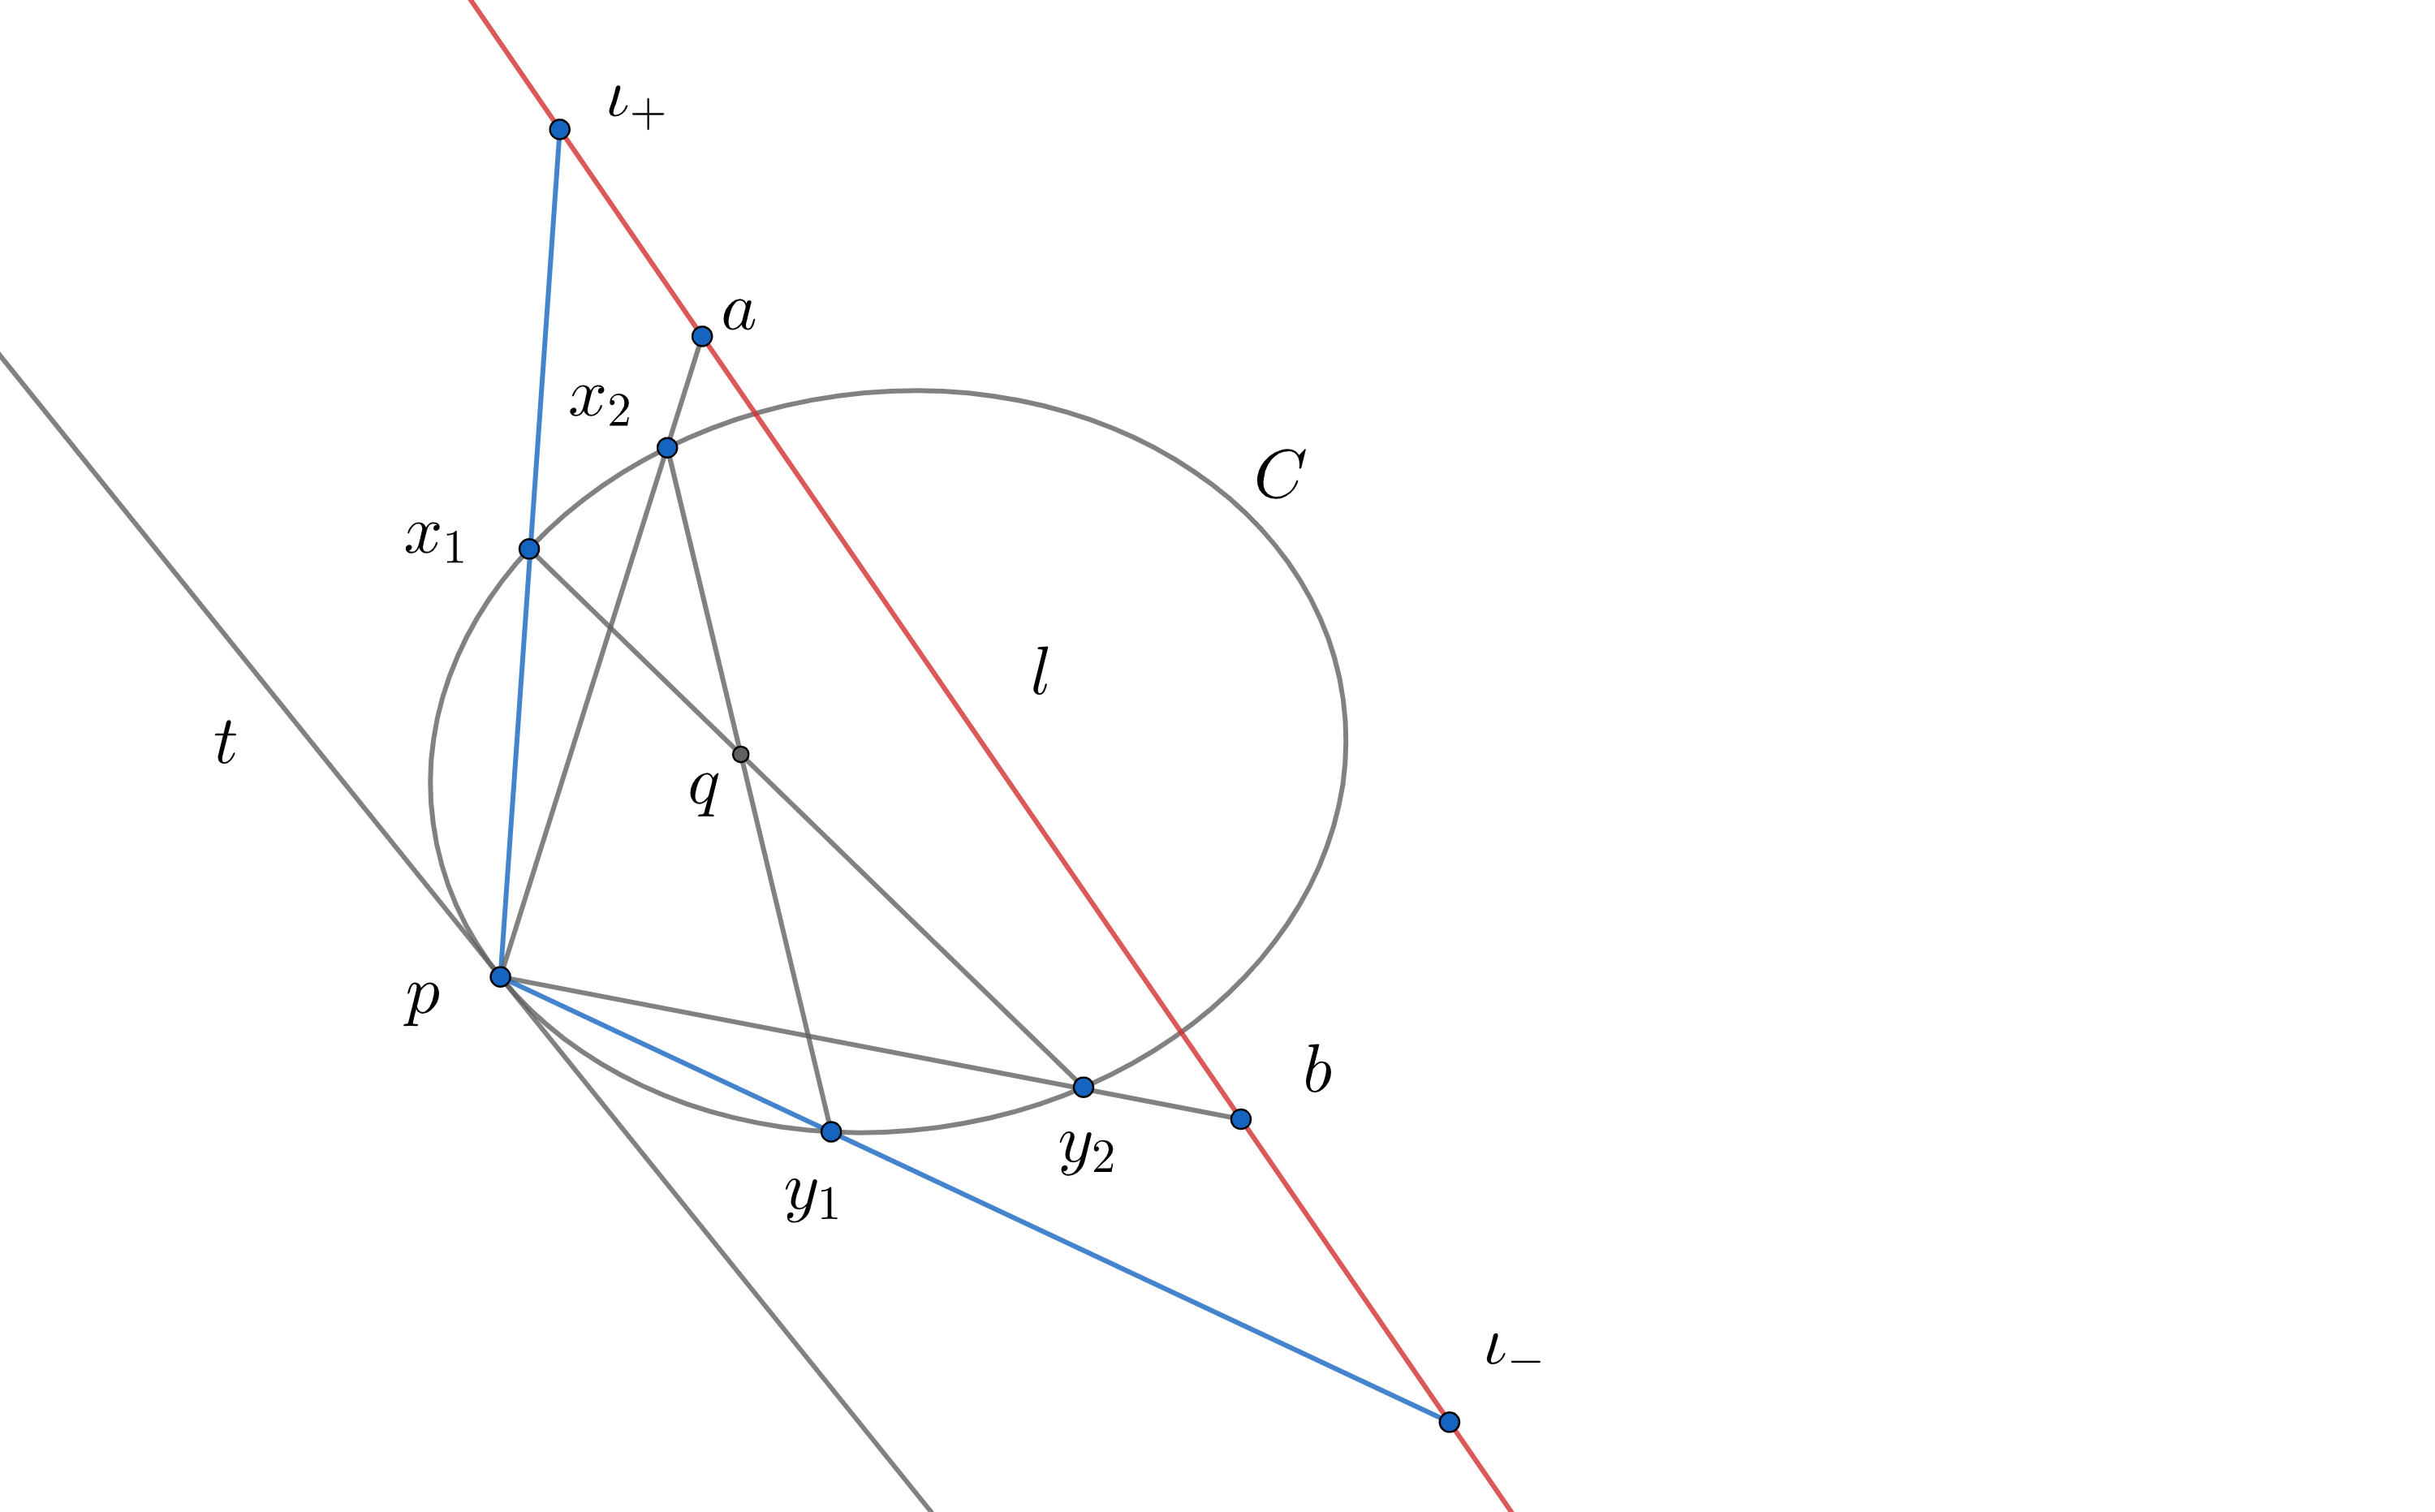
\includegraphics[width=0.6\linewidth]{pic29}
\end{figure}\\
Пусть $x_1=(p\iota_+)\cap C, y_1=(p\iota_-)\cap C$, а $\sigma (x) = y, \ x, y \in C$.\\
У инволюции есть центр, это $(x_1y_1)\cap(x_2y_2)$. Таким образом, все хорды пересекаются в точке $q$.\\
\\
Рассмотрим гомографию на конике $\upvarphi: p^\times \rightarrow q^\times$, $\upvarphi^2(px) = \upvarphi(xq) = px$ (обозначим $(px) \leftrightarrow (xq)$). Тогда если $(xq) \cap C = y$, то $(px) \leftrightarrow (py)$, следовательно $x \leftrightarrow y$, причем $(px) \perp (py)$.\\
\\
При $x=p \ (xq) = (pq)$, следовательно $p \leftrightarrow (pq) \cap C$ и $t, (pq)$ переставляются инволюцией, следовательно, они перпендикулярны.\\